\documentclass[14pt,usenames,dvipsnames]{beamer}
\usepackage[utf8]{inputenc}
\usefonttheme{structurebold}
\usepackage{cabin}



\usetheme{Madrid}
\usecolortheme{default}

\setbeamertemplate{section in toc}{\hspace*{1em}\inserttocsection}
\setbeamertemplate{subsection in toc}{\hspace*{2em}\inserttocsubsection}
%------------------------------------------------------------
%This block of code defines the information to appear in the
%Title page
\title[About Beamer] %optional
{A Secure Password Wallet based on the SEcube™ framework}


\author % (optional)
{Walter Gallego Gómez}

\institute[VFU] % (optional)
{
 Department of control and computer engineering\\
Politecnico di Torino
}

\date[VLC 2014] % (optional)
{July 23, 2018}

\titlegraphic{   \includegraphics[width=2cm]{logopolito}
   }

%\logo{
\includegraphics[height=1.5cm]{logo-polito}}

%End of title page configuration block
%------------------------------------------------------------



%------------------------------------------------------------
%The next block of commands puts the table of contents at the 
%beginning of each section and highlights the current section:

\AtBeginSection[]
{
  \begin{frame}
    \frametitle{Outline}
    \tableofcontents[currentsection]
  \end{frame}
}
%------------------------------------------------------------


\begin{document}

%gets rid of bottom navigation bar and adds numbers in custom size and color
\setbeamerfont{page number in head/foot}{size=\scriptsize}
\setbeamercolor{page number in head/foot}{fg=NavyBlue}
\setbeamertemplate{footline}[frame number]{}

%gets rid of navigation symbols
\setbeamertemplate{navigation symbols}{}

%The next statement creates the title page.
\frame{\titlepage}


\begin{frame}
\frametitle{Motivation}
The need for a hardware-based password manager is justified answering these three questions:


\begin{block}<2,3,8>{Are passwords still relevant?}
\onslide<3,8> {Yes, they are the dominant form of authentication.}
\end{block}

\begin{block}<4,5,8>{Why should people use password managers?}
\onslide<5,8> {So they can use unique strong passwords.}
\end{block}

\begin{block}<6,7,8>{Why are hardware-based approaches more reliable?}
\onslide<7,8> {Hardware approaches use two-factor authentication.}
\end{block}

%\begin{itemize}
%    \item<1-> Are passwords still relevant?
%    
%    \onslide<2> {Yes, dominant form of authentication}
%
%    \item<3-> Why should people use password managers?
%    
%   \onslide<4> {Yes, dominant form of authentication}
%
%    \item<5-> Why are hardware-based approaches more reliable?
%
%   \onslide<6> {Yes, dominant form of authentication}
%\end{itemize}

\end{frame}



%---------------------------------------------------------
%This block of code is for the table of contents after
%the title page
\begin{frame}
\frametitle{Outline}
\tableofcontents
\end{frame}
%---------------------------------------------------------


\section{Introduction}



\begin{frame}
\frametitle{Introduction}


\end{frame}



\section{Software and Hardware components}

%---------------------------------------------------------
%Highlighting text
\begin{frame}
\frametitle{Software Libraries}

The following open source libraries were used:

\begin{block}<2,3,10>{Qt: GUI and wrappers}
\onslide<3,10> {Compatible with C/C++, Cross-platform}
\end{block}

\begin{block}<4,5,10>{SQLite: DataBase management}
\onslide<5,10> {Self-contained...}
\end{block}

\begin{block}<6,7,10>{PwGen: Password generator}
\onslide<7,10> {Strong Random or readable}
\end{block}

\begin{block}<8,9,10>{zxcvbn: Password strength estimator}
\onslide<9,10> {Considers a lot of cases....}
\end{block}
\end{frame}

\begin{frame}
\frametitle{SEcube™ APIs hierarchy}
\begin{center}
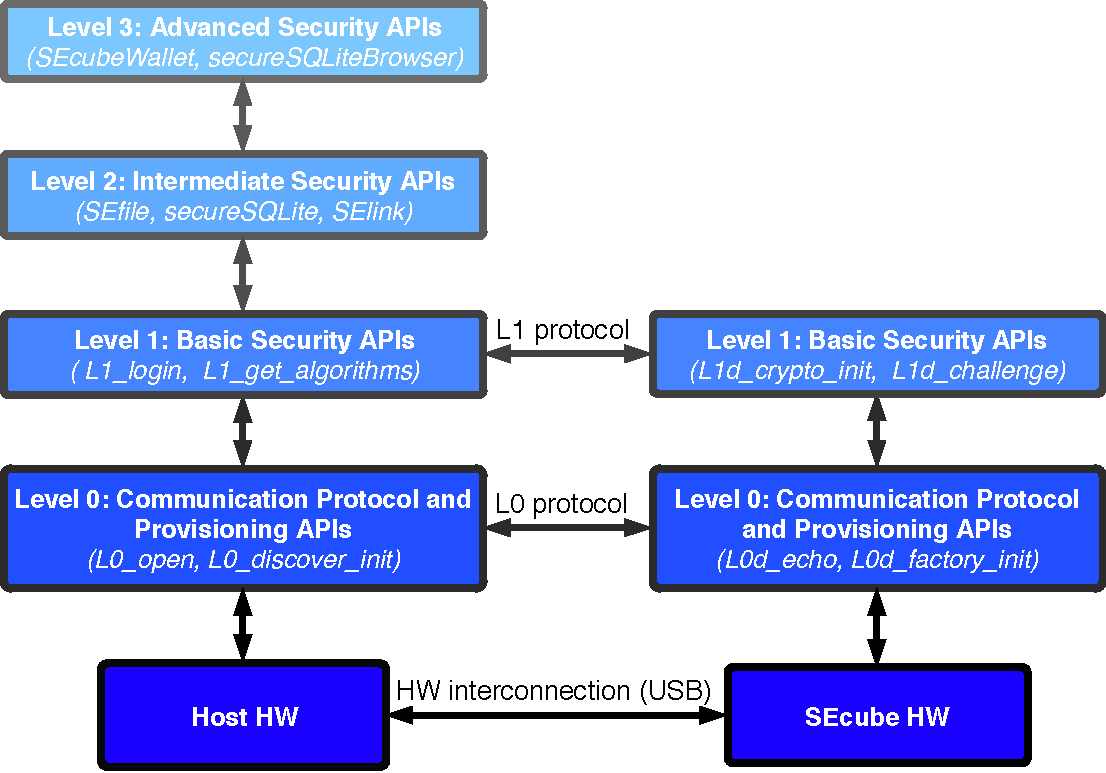
\includegraphics[width=\textwidth,height=0.85\textheight,keepaspectratio]{levels}
\end{center}
\end{frame}

\section{Design}

\begin{frame}
\only<1>{\frametitle{SEcubeWallet Application}}
\only<2>{\frametitle{Open device and authenticate}}
\only<3>{\frametitle{Create In-memory Wallet}}
\only<4>{\frametitle{Generate Password/Passphrase}}
\only<5>{\frametitle{Evaluate Strength}}
\only<6>{\frametitle{Encrypt and Save Wallet to disk}}
\only<7>{\frametitle{General Architecture}}
\begin{center}
\includegraphics<1>[width=\textwidth,height=0.85\textheight,keepaspectratio]{BasicDesignOnly}
\includegraphics<2>[width=\textwidth,height=0.85\textheight,keepaspectratio]{BasicDesignLog}
\includegraphics<3>[width=\textwidth,height=0.85\textheight,keepaspectratio]{BasicDesignInMem}
\includegraphics<4>[width=\textwidth,height=0.85\textheight,keepaspectratio]{BasicDesignGen}
\includegraphics<5>[width=\textwidth,height=0.85\textheight,keepaspectratio]{BasicDesignZ}
\includegraphics<6>[width=\textwidth,height=0.85\textheight,keepaspectratio]{BasicDesignDisk}
\includegraphics<7>[width=\textwidth,height=0.85\textheight,keepaspectratio]{BasicDesign}

\end{center}
\end{frame}


%In this slide, some important text will be
%\alert{highlighted} beause it's important.
%Please, don't abuse it.
%
%\begin{block}{Remark}
%Sample text
%\end{block}
%
%\begin{alertblock}{Important theorem}
%Sample text in red box
%\end{alertblock}
%
%\begin{examples}
%Sample text in green box. "Examples" is fixed as block title.
%\end{examples}
%\end{frame}
%---------------------------------------------------------


%---------------------------------------------------------
%Two columns
%\begin{frame}
%\frametitle{Two-column slide}
%
%\begin{columns}
%
%\column{0.5\textwidth}
%This is a text in first column.
%$$E=mc^2$$
%\begin{itemize}
%\item First item
%\item Second item
%\end{itemize}
%
%\column{0.5\textwidth}
%This text will be in the second column
%and on a second tought this is a nice looking
%layout in some cases.
%\end{columns}
%\end{frame}
%---------------------------------------------------------


\end{document}